\section{Results on ECUs}

\subsection{Coverages and request savings}

\subsubsection{New service scan approaches}

% RC service

\begin{table}[h]
    \begin{center}
    \begin{tabular}{ccc}
        \hline
        & \textbf{Coverage} & \textbf{Speed-up} \\
        \hline
        \textbf{audi\_cgw} & 87.6\% & 65.4\% \\
        \textbf{bfft-ecu} & 100\% & 66.2\% \\
        \textbf{bmw-gateway-ecu-bdc} & 100\% & 66.2\% \\
        \textbf{bmw-gateway-ecu-zgw} & 100\% & 64.5\% \\
        \textbf{bmw-gateway-ecu2} & 100\% & 64.6\% \\
        \textbf{bmw-tcu} & 100\% & 66.7\% \\
        \textbf{bosch-ecu} & 100\% & 64.6\% \\
        \textbf{dashboard} & 50.0\% & 66.2\% \\
        \textbf{mercedes-ezs} & 100\% & 65.1\% \\
        \textbf{seppmed} & 100\% & 66.2\% \\
        \textbf{tesla-airbag-ecu} & 100\% & 66.7\% \\
        \hline

    \end{tabular}
    \end{center}
    \caption{Measured coverages and speed-ups on ECUs with approach 1 for the RC service.}
    \label{tab:evaluation-approach1}
\end{table}

9 of 11 ECUs had a full coverage. The coverage for the dashboard ECU notable low. Therefore, a closer look was taken there. It turned out that the Dashboard only supports two identifiers. The identifier 515 for Type1 and identifier 61,728 for Type3. The former is detected, but the resulting range for Type3 is far from the identifier 61,728. Hence, the loss and a coverage of 50\%.

The speed-up is calculated by comparing the number of requests sent with the selective enumerator and the number of requests that would have been sent with the old enumerator for an entire scan. For each ECU it is close to the theoretical maximum of $66.\overline{6}$ \%, leading to the evaluation that there is a great potential in this approach.

This approach is applicable to scans of services with multiple fields, as it is the case with the RC service that has the \mintinline{text}{routineControlType} and \mintinline{text}{routineIdentifier} fields. This results in a high scan time for this service and thus a high time-saving potential. However, if an identifier is not recognized during the first scan, it will not be recognized in the next scans as well.


% RDBI service

\begin{table}[h]
    \begin{center}
    \begin{tabular}{ccc}
        \hline
        & \textbf{Coverage} & \textbf{Speed-up} \\
        \hline
        \textbf{audi\_cgw} & 87.8\% & 85.0\% \\
        \textbf{bfft-ecu} & 88.4\% & 96.6\% \\
        \textbf{bmw-gateway-ecu-bdc} & 100\% & 96.1\% \\
        \textbf{bmw-gateway-ecu-zgw} & 94.3\% & 95.8\% \\
        \textbf{bmw-gateway-ecu2} & 83.3\% & 96.1\% \\
        \textbf{bmw-tcu} & 72.2\% & 96.3\% \\
        \textbf{bosch-ecu} & 90.7\% & 93.3\% \\
        \textbf{dashboard} & 92.4\% & 94.4\% \\
        \textbf{mercedes-ezs} & 89.3\% & 94.7\% \\
        \textbf{seppmed} & 83.0\% & 95.9\% \\
        \textbf{tesla-airbag-ecu} & 100\% & 96.4\% \\
        \hline
    \end{tabular}
    \end{center}
    \caption{Measured coverages and speed-ups on ECUs with approach 2 for RDBI service.}
    \label{tab:evaluation-approach2}
\end{table}

\autoref{tab:evaluation-approach2} shows the resulting coverage and speed-ups for this approach for the RDBI service. It should be noted, that these values vary slightly for each run because a random scan is used.

Overall, the coverages are lower with this approach than for approach 1. Only for two ECUs a coverage of 100\% is reached. The speed-ups are high at approximately 95\%. Nevertheless, the speed-ups of approach 1 are higher in practice, because that approach can be applied to larger service scans, and then a speed-up of about 66\% saves more time there than a speed-up of 95\% here.

The biggest problem with this approach is the newly added random factor. The coverage can be great for one scan, but low for the next one. This would require performing multiple scans using the new implementation to ensure that most identifiers were found.

\subsubsection{Not scanning unsupported services}

\autoref{fig:serviceNotSupported-savings} illustrates the number of saved packets for each ECU with this approach. It is only an approximation because for this graph, the responses with the both described NRCs have been counted. Of course, not every response can be saved with these NRCs, since at least one request must first be made to see the NRC of that service for a state. But this number of requests, as described in the previous paragraph, is low and negligible, especially considering that the minimum value of saved requests is about 70,000.

\begin{figure}[h]
    \centering
    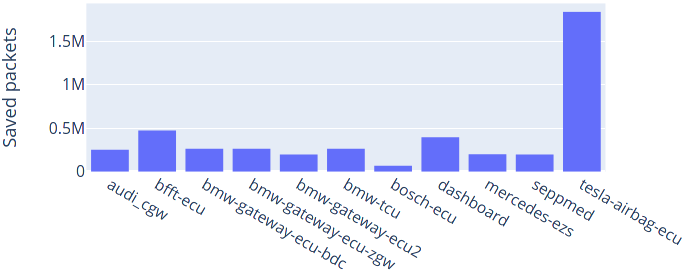
\includegraphics[width=0.8\textwidth]{serviceNotSupported-savings}
    \caption{Saved number of requests with this approach (approx).}
    \label{fig:serviceNotSupported-savings}
\end{figure}

There is a potential problem with this approach. Reliance is placed on the manufacturer to properly implement these NRCs. It is conceivable that the ECU responds to an identifier with 0x11 or 0x7f, although a subsequent identifier would actually have been answered positively. The occurrences of this behavior are shown in \autoref{fig:serviceNotSupported-losses}. It was calculated by evaluating the responses for each enumerator for each state. Once a negative response with NRC 0x11 or 0x7f was received, an internal counter was incremented with each subsequent positive response.
And in comparison to the potential savings (\autoref{fig:serviceNotSupported-savings}), the losses are negligible.

\begin{figure}[H]
    \centering
    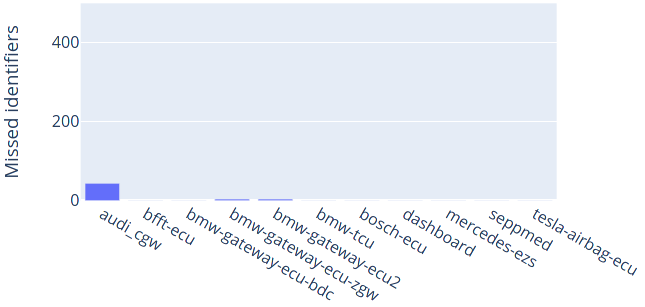
\includegraphics[width=0.8\textwidth]{serviceNotSupported-losses}
    \caption{Lost number of positive responses with this approach.}
    \label{fig:serviceNotSupported-losses}
\end{figure}

Avoiding scanning unsupported services is the safest way to save time of all three approaches. It is unlikely that identifiers will be missed, but the speed gain can still be high.

\subsection{Actual time savings}

For each ECU, the same scans as for gathering information and profiling were executed again, they differ only in the use of the new implementations.

\begin{figure}[h]
    \centering
    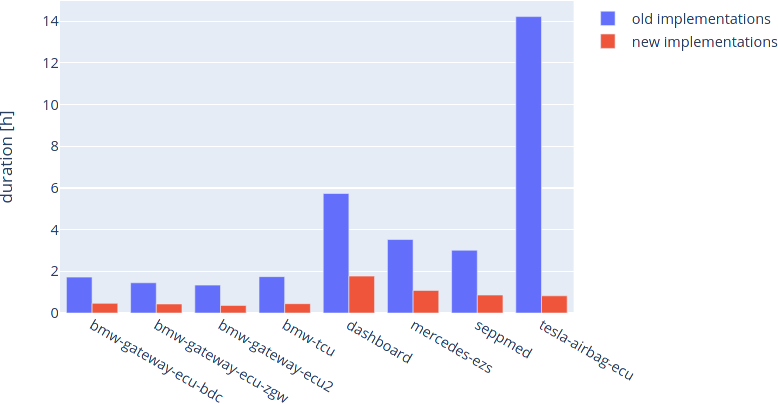
\includegraphics[width=1\textwidth]{durations-diff}
    \caption{Observed runtimes for a UDS scan with new implementations.}
    \label{fig:durations-diff}
\end{figure}

As \autoref{fig:durations-diff} illustrates, the speed-up is severe, especially for the Tesla ECU, which has a relatively high average response time (about 0.02 seconds) compared to the others (0.001 to 0.008 seconds).
Three ECUs are excluded from this observation because they were no longer available at the time of re-evaluating the scan durations.
